\chapter{Marco teórico}
\label{ch:marco}


En este cap\'itulo se detalla el contenido te\'orico necesario para el desarrollo de este trabajo. La propuesta consiste en la optimizaci\'on y paralelizaci\'on del filtro Deceived Non-Local Means (DNLM). Este filtro es una modificaci\'on del filtro Non-Local Means (NLM) que adiciona la mejora de bordes y contraste, conservando la buena respuesta del filtro NLM en cuanto a preservaci\'on de bordes y robustez ante el ruido \cite{calderon2015dewaff}. La propuesta de paralelizaci\'on incluye la evaluaci\'on de optimizaciones computacionales exactas desarrolladas originalmente para el filtro NLM y adaptadas en este trabajo al filtro DNLM. Las optimizaciones computacionales del filtro NLM se pueden agrupar en dos enfoques: Optimizaciones exactas y aproximaciones del algoritmo.  En este trabajo se limita al estudio de optimizaciones exactas al filtro NLM debido a la necesidad de obtener la mejor calidad del filtro. Existen mejoras en el rendimiento del filtro NLM en t\'erminos del ruido eliminado, sin embargo se emplean t\'ecnicas de cl\'ustering, diccionarios y otros m\'etodos para preclasificar parches similares en la imagen, a\~nadiendo complejidad computacional al filtro \cite{pardoNLM:2018,Chan2013,Tasdizen2009,Chatterjee2008,JI20091238,Karam2018}. 



\section{Eliminaci\'on de ruido}

\subsection{Ruido Blanco Aditivo de distribuci\'on Gaussiana}
\label{ch:marco_agwn}

El ruido presente en im\'agenes se debe a fen\'omenos naturales en el proceso de captura, transmisi\'on y almacenamiento de las im\'agenes. 	Una forma de modelar este ruido es mediante el ruido blanco aditivo de distribuci\'on gaussiana. Este ruido es llamado gaussiano porque se manifiesta en funci\'on de una distribuci\'on de probabilidad gaussiana. Se dice que es blanco porque el espectro de intensidad es plano. Se le llama aditivo porque se encuentra acumulado los pixeles de la imagen. El modelo Gaussiano se considera como el m\'as adecuado para la representaci\'on de ruido en im\'agenes y est\'a dado por la ecuaci\'on \ref{eq:modelruido}.

\begin{equation}
\label{eq:modelruido}
U = X + V
\end{equation}

 donde $X$ corresponde a la imagen sin ruido y el t\'ermino $V$ corresponde a la Funci\'on de Densidad de Probabilidad Gaussiana dada en (\ref{eq:probfuncgauus}).

\begin{equation}
\label{eq:probfuncgauus}
P(V(x)) = \frac{1}{{\sigma \sqrt {2\pi } }}e^{{{ - \left( {V(x) - \mu } \right)^2 } \mathord{\left/ {\vphantom {{ - \left( {x - \mu } \right)^2 } {2\sigma ^2 }}} \right. \kern-\nulldelimiterspace} {2\sigma ^2 }}}
\end{equation}

El par\'ametro $\sigma$ es la desviaci\'on est\'andar  y $\mu$ el valor medio de la distribuci\'on de probabilidad.


\subsection{Filtro Non-Local Means}
\label{ch:marco_nlm}

El filtro NLM forma parte de los filtros espaciales de promedio ponderado que pueden definirse de manera general como se detalla en (\ref{eq:weighted}).

\begin{equation}
\label{eq:weighted}
Y(U,p,m)=\left(\sum_{m\in \Omega}\psi_{i}\left(U, p, m\right)\right)^{-1} \\ \left(\sum_{m\in \Omega}\psi_{i}\left(U, p, m\right)U(m)\right),
\end{equation}

Donde $p$ y $m$ son pixeles contenidos en una ventana deslizante $\Omega$ de la imagen de entrada $U$ \cite{calderon2015dewaff}.

El filtro NLM se define mediante la funci\'on de pesado $\psi$ utilizando la distancia Euclidiana para determinar la similitud entre vecindarios de dos pixeles $p$ y $m$. De esta manera se determina el peso en la contribuci\'on para el ponderamiento de los pixeles en una regi\'on dada por una ventana $\Omega$. 

Este filtro introduce el concepto de similitud entre vencindarios de pixeles y no entre sus intensidades como otros filtros. Este enfoque reduce los cambios bruscos en la intensidad de pixeles aleda\~nos comparando los vecindarios en un \'area local, a la vez que permite conservar detalles como bordes y patrones en la imagen\cite{calderon2015dewaff}. La ecuaci\'on (\ref{eq:nlmfunc}) muestra la funci\'on de pesado del filtro NLM.

\begin{equation}
\label{eq:nlmfunc}
\[
\psi_{\textrm{NLM}}\left(p,m\right)=\exp\left(-\frac{\left\Vert \vec{\eta}\left(\omega,m\right)-\vec{\eta}\left(\omega,p\right)\right\Vert }{\sigma^{2}}\right).
\]
\end{equation}

Donde $\sigma$ es el par\'ametro que controla el grado de suavizado del filtro y $\vec{\eta}$ el vector que contiene todos los pixeles del vecindario $\omega$.

En cuanto a la complejidad computacional del filtro, para el peor escenario de usar una ventana $|\Omega| = S\timesS$ y un vecindario de $|\omega| = P\timesP$ pixeles, la complejidad computacional del filtro DNLM es de $O(S^2 \cdot P^2 \cdot N \cdot M)$, donde $N\timesM$ corresponde a el n\'umero total de pixeles de la imagen de entrada $U$. 



\subsection{Mejora de bordes y contraste}

\subsubsection{Unsharp Masking}
\label{ch:marco_usm}

Los m\'etodos de Unsharp Masking se utilizan para el realce de los bordes y la mejora de contraste en las im\'agenes. Se realiza mediante una substracci\'on de la imagen suavizada a la imagen original. Esto origina una imagen $B$ con las frecuencias altas de la imagen, es decir, los bordes y otros cambios de intensidad bruscos en los pixeles t\'ipicamente representados como detalles y ruido. 

Adicionalmente, se puede emplear un enfoque inverso que consiste en sumar la imagen $B$ con la informaci\'on de bordes y detalles en alta frecuencia a la imagen original. La adici\'on se controla en una proporci\'on dada por el coeficiente $\lambda$, como se observa en (\ref{eq:unsharpmask}). La imagen $B$ se obtiene por medio de la convoluci\'on entre la imagen original y un kernel de aproximaci\'on a la segunda derivada, como el kernel Laplaciano, Laplaciano de Gaussiano o de diferencia Gaussiana.

\begin{equation}
\label{eq:unsharpmask}
G=U+\lambda\,B
\end{equation}

donde $B$ corresponde a

\begin{equation}
\label{eq:unsharfilter}
B=l*U
\end{equation}

y $l$ puede estar dado por:

\begin{equation} l = \left[
\begin{array}{ccc}
1 & 1 & 1\\
1 & -8 & 1\\
1 & 1 & 1
\end{array}\right]
\end{equation}

para el caso de la aproximaci\'on b\'asica a la segunda derivada.

En este trabajo se utiliza un kernel de aproximaci\'on a la segunda derivada por medio del Laplaciano del Gaussiano \cite{sotak1989laplacian}, como se define en (\ref{eq:log}):

\begin{equation}
\label{eq:log}
\operatorname{LoG}(x,y) = \frac{1}{\pi\sigma^4}\left(\frac{x^2+y^2}{2\sigma^2} - 1\right)e^{-\frac{x^2+y^2}{2\sigma^2}},
\end{equation}



\subsection{Filtro Deceived Non-Local Means}
\label{ch:marco_dnlm}


El enfoque del filtro Deceived Non-Local Means (DNLM) consiste en la combinaci\'on de un m\'etodo de Undsharp Masking (USM) con el filtro NLM, con el prop\'osito de lograr por un lado una mejora en los bordes y en el contraste de la imagen, y por otro lado la eliminaci\'on del ruido Gausiano  presente en la imagen. La combinaci\'on propuesta se basa en el desacople entre la imagen usada en el pesado (imagen original $U$) y la utilizada en el filtrado $U_{USM}$. Esto permite evitar el efecto anillo presente en las im\'agenes filtradas con el USM \cite{calderon2015dewaff}.

 La ecuaci\'on (\ref{eq:dnlm}) presenta la definici\'on del enfoque de desacoplamiento del filtro.

\begin{equation}
\label{eq:dnlm}
Y(p)=\left(\sum_{m\in \Omega}\psi_{NLM}\left(U, p, m\right)\right)^{-1} \\ \left(\sum_{m\in \Omega}\psi_{NLM}\left(U, p, m\right)U_{USM}(m)\right),
\end{equation}




\subsection{Optimizaciones computacionales}
\label{ch:marco_opt}

\subsubsection{DNLM-IIFFT}
\label{ch:marco_dnlmifft}

Esta optimizaci\'on computacional utiliza im\'agenes integrales y la transformada r\'apida de fourier para disminuir la complejidad computacional del algoritmo. 



Al analizar la distancia Euclidiana entre los vecindarios $D$,

\begin{equation}
D\left(p,m\right)=\left\Vert \vec{\eta}\left(\omega,m\right)-\vec{\eta}\left(\omega,p\right)\right\Vert
\end{equation}

\begin{equation}
D\left(p,m\right)=\sum_{u}\left(\varPhi_{m}\left(u\right)-\varPhi_{p}\left(u\right)\right)^{2} \enspace ,
\end{equation}
 donde $\sum_{u}$ denota la sumatoria de los valores dados por la diferencia entre los vecindarios $\varPhi_m$ and $\varPhi_p$.

Al desarrollar la diferencia cuadrada y al reescribir los t\'erminos cuadr\'aticos como $\varPhi_{m}^{2}=\sum_{u}\varPhi_{m}\left(u\right)^{2} \enspace$,  se obtiene: 
\begin{equation}
 D\left(m,p\right)=\varPhi_{m}^{2}-2\sum_{u}\varPhi_{p}\left(u\right)\varPhi_{m}\left(u\right)+\varPhi_{p}^{2}  \enspace ,
 \label{eq_cuadratica}
\end{equation}


\begin{equation}
D\left(m,p\right)=\varPhi_{m}^{2}-2\varPhi_{p}\cdot\varPhi_{m}+\varPhi_{p}^{2} \enspace ,
\end{equation}
donde $\varPhi_{p}\cdot\varPhi_{m}$ corresponde al producto punto entre matrices. El siguiente ejemplo ilustra el c\'alculo de la distancia Euclideana entre los vecindarios de pixeles contenidos en la imagen $U\in\mathbb{R}^{5\times5}$ definida en la Tabla \ref{tab_ImageExample}.








\begin{table}
\begin{center}
\caption{Ejemplo de imagen $U$.}

\renewcommand{\arraystretch}{1.4}
\setlength\tabcolsep{3pt}

{
\begin{tabular}{cc|ccc|c}
 & \multicolumn{1}{c}{\textbf{1}} & \textbf{2} & \textbf{3} & \multicolumn{1}{c}{\textbf{4}} & \textbf{5}\tabularnewline
\textbf{1} & \multicolumn{1}{c}{5} & 12 & 1 & \multicolumn{1}{c}{3} & 2\tabularnewline
\cline{3-5} 
\textbf{2} & 5 & 2 & 3 & 1 & 4\tabularnewline
\textbf{3} & 3 & 1 & \textbf{2} & 3 & 1\tabularnewline
\textbf{4} & 4 & 3 & 2 & 1 & 3\tabularnewline
\cline{3-5} 
\textbf{5} & \multicolumn{1}{c}{1} & 5 & 6 & \multicolumn{1}{c}{5} & 3\tabularnewline
\end{tabular}
}
\par\end{center} \label{tab_ImageExample}
\end{table}




Para efectos de la ilustraci\'on, se toma una ventana $\Omega_{\left(3,3\right)}\in\mathbb{R}^{3\times3}$  y se realiza  el c\'alculo de la distancia Euclidiana entre los vecindarios $\varPhi_{\left(3,3\right)}$ y $\varPhi_{\left(2,2\right)}$:

\begin{equation}
\label{eq:resultado1}
\begin{array}{c}
\left\Vert \varPhi_{\left(3,3\right)}-\varPhi_{\left(2,2\right)}\right\Vert ^{2}=\left\Vert \begin{array}{ccc}
2 & 3 & 1\\
1 & 2 & 3\\
3 & 2 & 1
\end{array}-\begin{array}{ccc}
5 & 12 & 1\\
5 & 2 & 3\\
3 & 1 & 2
\end{array}\right\Vert\end{array}
=10.3923^{2}=108 \enspace .
\end{equation}



 Dado el desarrollo de la diferencia cuadr\'atica entre los vecindarios en la parte derecha de la ecuaci\'on, se puede obtener el c\'alculo utilizando la imagen integral de la matriz conformada por la operaci\'on cuadr\'atica de los elementos de la matriz $U\in\mathbb{R}^{5\times5}$. De esta manera permite calcular la distancia Euclideana para obtener: 
\begin{equation}
\left\Vert \varPhi_{\left(3,3\right)}-\varPhi_{\left(2,2\right)}\right\Vert =\varPhi_{\left(3,3\right)}^{2}-2\varPhi_{\left(2,2\right)}\cdot\varPhi_{\left(3,3\right)}+\varPhi_{\left(2,2\right)}^{2} 
\end{equation}


\begin{equation}
=\sum\left(\begin{array}{ccc}
4 & 9 & 1\\
1 & 4 & 9\\
9 & 4 & 1
\end{array}\right)-2\left(\begin{array}{ccc}
2 & 3 & 1\\
1 & 2 & 3\\
3 & 2 & 1
\end{array}\cdot\begin{array}{ccc}
5 & 12 & 1\\
5 & 2 & 3\\
3 & 1 & 2
\end{array}\right)
+\sum\left(\begin{array}{ccc}
25 & 144 & 1\\
25 & 4 & 9\\
9 & 1 & 4
\end{array}\right)
\end{equation}



\begin{equation}
=42+-2\cdot78+222=42-156+222=108\label{eq:cuadrados-1} \enspace ,
\end{equation}
consistente con los resultados obtenidos en (\ref{eq:resultado1}).




La optimizaci\'on de este algoritmo se centra en el c\'alculo de la distancia Euclidiana definida en  (\ref{eq_cuadratica}) de la siguiente manera:
\begin{itemize}
\item El uso de la imagen integral cuadrada para calcular los t\'erminos $\varPhi_{i}^{2}$
y $\varPhi_{j}^{2}$.
\item Calcular la Transformada de Fourier para obtener el t\'ermino $-2\varPhi_{j}\cdot\varPhi_{i}$
correspondiente a la autocorrelaci\'on con la se\~nal
$\varPhi_{j}$.
\end{itemize}
 
\paragraph{I\'agenes integrales}


La imagen integral $I$ es definida en \cite{viola2001robust}, con una notaci\'on de barrido por pixel $i=(x,y)$, dada por: 
\begin{equation}
I_{\Sigma}\left(x,y\right)=\sum_{u\leq x,v\leq y}I\left(u,v\right) \enspace ,
\end{equation}
la cual corresponde a la sumatoria de los  pixeles ubicados a la izquierda y superiores al pixel $i=(x,y)$.
Continuando con el ejemplo previamente mostrado, la imagen integral para la matriz $U$ con sus elementos al cuadrado se calcula como se muestra en la Tabla \ref{tab_ImagenesIntegrales}. 
\begin{table}
\caption{Imagen integral para $U^2$.}
\begin{center}
\renewcommand{\arraystretch}{1.4}
\setlength\tabcolsep{3pt}


{
\begin{tabular}{cc|ccc|c}
 & \multicolumn{1}{c}{\textbf{1}} & \textbf{2} & \textbf{3} & \multicolumn{1}{c}{\textbf{4}} & \textbf{5}\tabularnewline
\textbf{1} & \multicolumn{1}{c}{\textbf{25(A)}} & 169 & 170 & \multicolumn{1}{c}{\textbf{179(B)}} & 183\tabularnewline
\cline{3-5} 
\textbf{2} & 50 & 198 & 208 & 218 & 238\tabularnewline
\textbf{3} & 59 & 208 & \textbf{222} & 241 & 262\tabularnewline
\textbf{4} & \textbf{75(C)} & 233 & 251 & \textbf{271(D)} & 301\tabularnewline
\cline{3-5} 
\textbf{5} & \multicolumn{1}{c}{76} & 259 & 313 & \multicolumn{1}{c}{358} & 397\tabularnewline
\end{tabular}
}


\par\end{center}
\label{tab_ImagenesIntegrales}
\end{table}
Para un c\'alculo eficiente de la sumatoria del \'area de una regi\'on de la imagen, se debe notar que: 
\begin{equation}
I_{\Sigma}\left(x,y\right)=I\left(x,y\right)-I_{\Sigma}\left(x-1,y-1\right)+I_{\Sigma}\left(x,y-1\right)
\\+I_{\Sigma}\left(x-1,y\right) \enspace ,
\end{equation}
lo cual, para el ejemplo anterior significa:
\begin{equation}
I_{\Sigma}\left(3,3\right)=4-198+208+208=222 \enspace .
\end{equation}
Al utilizar la imagen integral para calcular la sumatoria de una regi\'on de la imagen original, limitada por los pixeles $A=\left(x_{0},y_{0}\right)$,
$B=\left(x_{1},y_{0}\right)$, $C=\left(x_{0},y_{1}\right)$ and $D=\left(x_{1},y_{1}\right)$, como se ilustra en la Tabla \ref{tab_ImagenesIntegrales}, se calcula de la siguiente manera: 

\begin{equation}
\sum_{x_{0}<x\leq x_{1},y_{0}<y\leq y_{1}}I\left(x,y\right)=I\left(D\right)+I\left(A\right)-I\left(B\right)-I\left(C\right) \enspace ,
\end{equation}
y para el ejemplo presentado para una ventana de dimensiones $3\times3$ alrededor del pixel $(3,3)$ los pixeles de las esquinas est\'an dados por: $A=\left(1,1\right)$, $B=\left(4,1\right)$,
$C=\left(1,4\right)$ y $D=\left(4,4\right)$, como se especifica en la Tabla \ref{tab_ImagenesIntegrales}. De esta manera, el c\'alculo de la sumatoria de los pixeles en una ventana est\'a dada por: 

\begin{equation}
\sum_{x_{0}<x\leq x_{1},y_{0}<y\leq y_{1}}I\left(3,3\right)=271+25-179-75=42 \enspace ,
\end{equation}

con lo cual, es consistente con el primer t\'ermino en (\ref{eq:cuadrados-1}). 

La incorporaci\'on de la imagen integral para la sumatoria del \'area de una ventana para una imagen de entrada con $N\timesM$ pixeles, presenta una complejidad computacional de $O(c)$, y s\'olamente debe ser calculada una vez en el filtro DNLM.


\paragraph{Transformada R\'apida de Fourier}

Como se monstr\'o anteriormente, el t\'ermino en la ecuaci\'on cuadr\'atica de la distancia Euclideana entre los vecindarios de los pixeles $i$ y $j$:
\begin{equation}
S\left(i,j\right)=N_{i}^{2}-2\sum_{a=0}^{m-1}\sum_{b=0}^{m-1}N_{j}\left(a,b\right)N_{i}\left(a,b\right)+N_{j}^{2} =N_{i}^{2}-2N_{j}\cdot N_{i}+N_{j}^{2} \enspace , 
\end{equation}


Los pesos son calculados



correspondiente al producto punto de las matrices $-2N_{j}\cdot N_{i}$,  puede ser calculado utilizando la FFT con una complejidad computacional logar\'itmica, reduciendo la funci\'on de costo del filtro DNLM a $O(S^2 \cdot log(P) \cdot N \cdot M)$



\subsubsection{Optimizaci\'on de Condat}
\label{ch:marco_condat}

Esta propuesta de optimizaci\'on al algoritmo NLM se caracteriza por su simpleza, al proponer un intercambio entre los loops de interaci\'on del algoritmo \cite{Condat2010}. La aceleraci\'on se consigue al incorporar convoluciones para realizar el ponderamiento de la ventana de b\'usqueda, operando sobre los valores producto de la diferencia cuadrada de los pixeles (\ref{eq:diffquad}) iterando las distancias entre los pixeles contenidos en la ventana de b\'usqueda \Omega \cite{Condat2010}. 

\begin{equation}
D\left(k\right) = \left(U\left(k + n\right) - U\left( k \right)\right)^2 ,
\label{eq:diffquad}
\end{equation}

y 

\begin{equation}
\label{eq:convmoas}
SSD = D * h ,
\end{equation}

donde se define la convoluci\on con un kernel $h$ (\ref{eq:convmoas}) que corresponde a un kernel de promediado.


La funci\'on de pesado resultante se muestra en la Ecuaci\'on (\ref{wmoas}). 

\begin{equation}
\[
\psi_{\textrm{DNLM-MOAS}}\left(k\right)=\exp\left(-\frac{ SSD\left(k\right) }{\sigma^{2}}\right).
\]
\label{eq:wmoas}
\end{equation}


Adem\'as plantea el aprovechamiento de la simetr\'ia presente en el c\'alculo de los pesos de los pixeles, consiguiendo una funci\'on de costo computacional de $O((2P + 2) \cdot (2S + 1)^2 \cdot N \cdot M)$.  





\subsection{Paralelizaci\'on}
\label{ch:marco_parallel}

Marco Teorico sobre paralelizacion.

\subsection{Arquitectura Intel Xeon Phi Knights Landing}
\label{ch:marco_xeonphi}

La arquitectura de procesador Intel Xeon Phi Knights Landing conocida como \textit{many-core} est\'a dise\~nada para aplicaciones de computaci\'on de alto rendimiento y es considerada la alternativa de Intel al desarrollo de algoritmos en GPU para prop\'osito general. A diferencia de la versi\'on anterior, esta nueva iteraci\'on con nombre clave Knights Landig permite el arranque de un sistema operativo por s\'i misma \cite{XeonPhiWhitePaper}. Posee de 32 a 36 celdas interconectadas por una interfaz de comunicaci\'on en 2D, cada una de ellas conformada por 2 CPUs y 1MB de Cach\'e L2 \cite{XeonPhiWhitePaper}. Cada uno de los CPUs incorpora 2 Unidades de Procesamiento Vectorial (VPU) con registros de hasta 512 bytes de largo \ref{XeonPhiWhitePaper}. 
Entre las caracter\'isticas que destacan del CPU es su modo de ejecuci\'on fuera de orden y el multihilo simult\'aneo de 4 hilos \cite{XeonPhiWhitePaper}. Una de sus particularidades es la incorporaci\'on de 16GB de Memoria de Alto Ancho de Banda (HBM) de hasta $450 Gbyte/s$ en el mismo chip como lo muestra la Figura \ref{fig:cpu_phi}, permitiendo tiempos de latencia cortos en comparaci\'on con los obtenidos con tecnolog\'ias DDR4 \cite{XeonPhiWhitePaper}.

\begin{figure}[H]
\centering
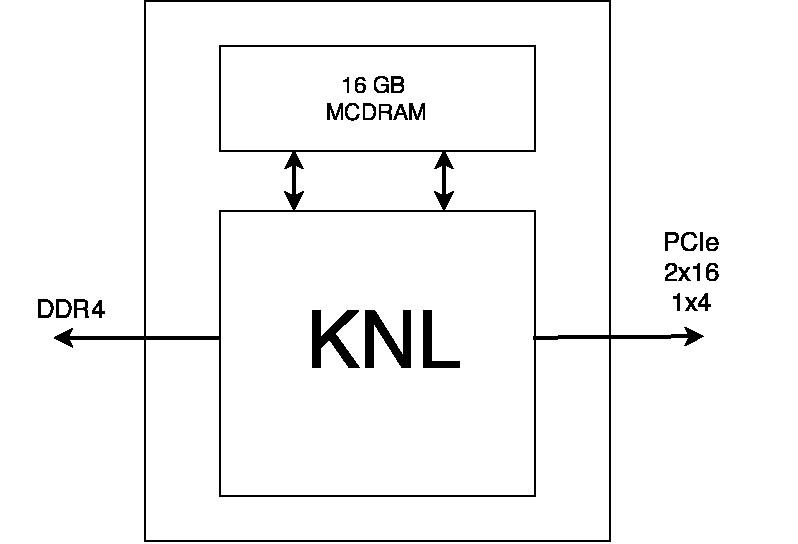
\includegraphics[width=0.5\textwidth]{fig/cpu}
\caption{Diagrama de alto nivel del procesador Xeon Phi KNL.}
\label{fig:cpu_phi}
\end{figure}


La memoria Cach\'e L2 es unificada de 1Mb compartida para los dos n\'ucleos que conforman cada celda \cite{XeonPhiWhitePaper}.
